\chapter{Design and Implementation}
\begin{quote} 
\it This chapter covers the implementation details of the concept, the algorithms. All the simulations were first carried out in MATLAB{\textregistered} and Simulink{\textregistered}, testing and verifying; then implementing the same in Hardware.
\end{quote}


\section{Cell Characterisation}
In this section, Model of two types of cells (\ac{a-Si} and \ac{DSCs}) is discussed.There are several Models that have been analysed in literature which are usually variations of the Single Diode model or the Double Diode model (discussed in section \ref{sec:SDM},\ref{sec:DDM} and \ref{sec:eDDM}).
 
\subsection{Test Setup}
in **furtherance of** creating a working solar cell model and to validate the algorithm several measurements would need to be performed. The Test-rig consisted of a blacked out enclosure to prevent **interference** from ambient light. The Test-rig is fitted with an array of evenly spaced White-\ac{LED}s to provide uniform illumination on the Test subject. The \ac{LED}-array are calibrated and temperature controlled so as to provide white light with a known spectra. A high precision Lux Meter(\textit{GOSSEN Mavolux 5032B}) is used to measure the  intensity of the light, as perceived by the human eye.The Light chamber is also routinely calibrated against a reference cell to factor-in the variations and degradation of the \ac{LED}s. The intensity of light is varied using a High-Voltage power source.A pictorial representation of the above description can be seen is figure  ~\ref{fig:test setup} on page ~\pageref{fig:test setup}. \\

 \begin{figure}[H]
  \begin{center}
  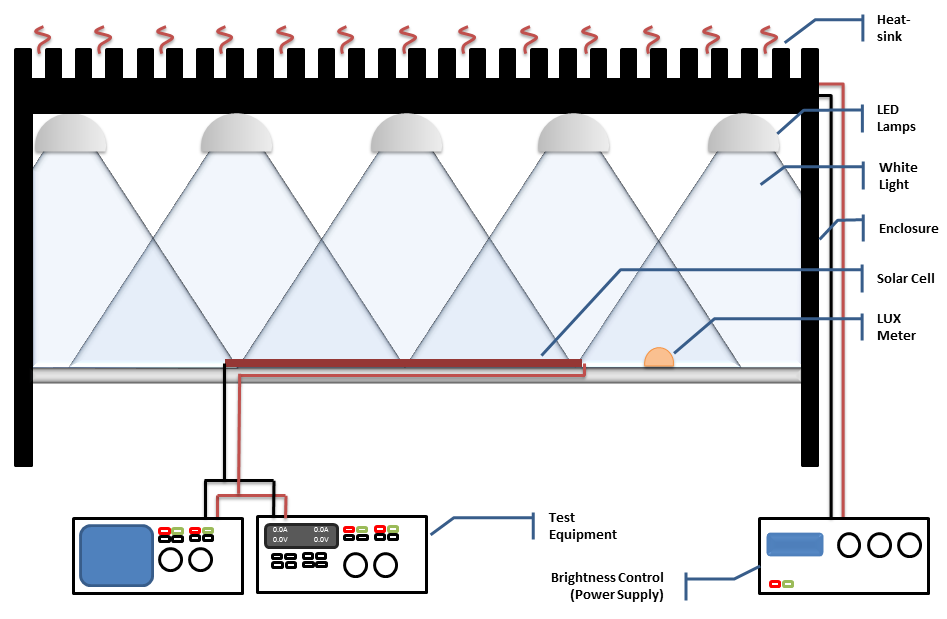
\includegraphics[width=\textwidth]{images/Light_Box}
  \caption{Test Setup }
  \label{fig:test setup}
  \end{center}
  \end{figure}
As the Sink Voltage is increased in small steps from 0 V to V\textsubscript{OC} and beyond the cell is forced to operate at the Sink Voltage resulting in the I-V graph depicted in figure ~\ref{fig:2500luxIV} on page ~\pageref{fig:2500luxIV}.
When the above is repeated for several different light intensities we get a three-dimensional surface shown in figure ~\ref{fig:luxIV100_2500} on page ~\pageref{fig:luxIV100_2500}\\

 \begin{figure}[H]
  \begin{center}
  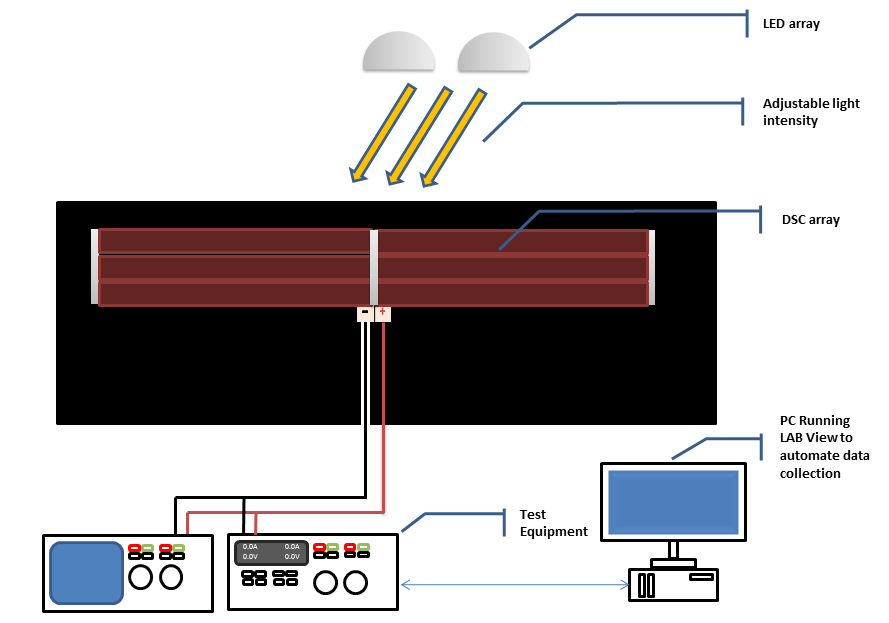
\includegraphics[width=\textwidth]{images/Cell_under_test}
  \caption{Cell Characterisation }
  \label{fig:Cell_U_test}
  \end{center}
  \end{figure}

  \begin{figure}[H]
  \begin{center}
  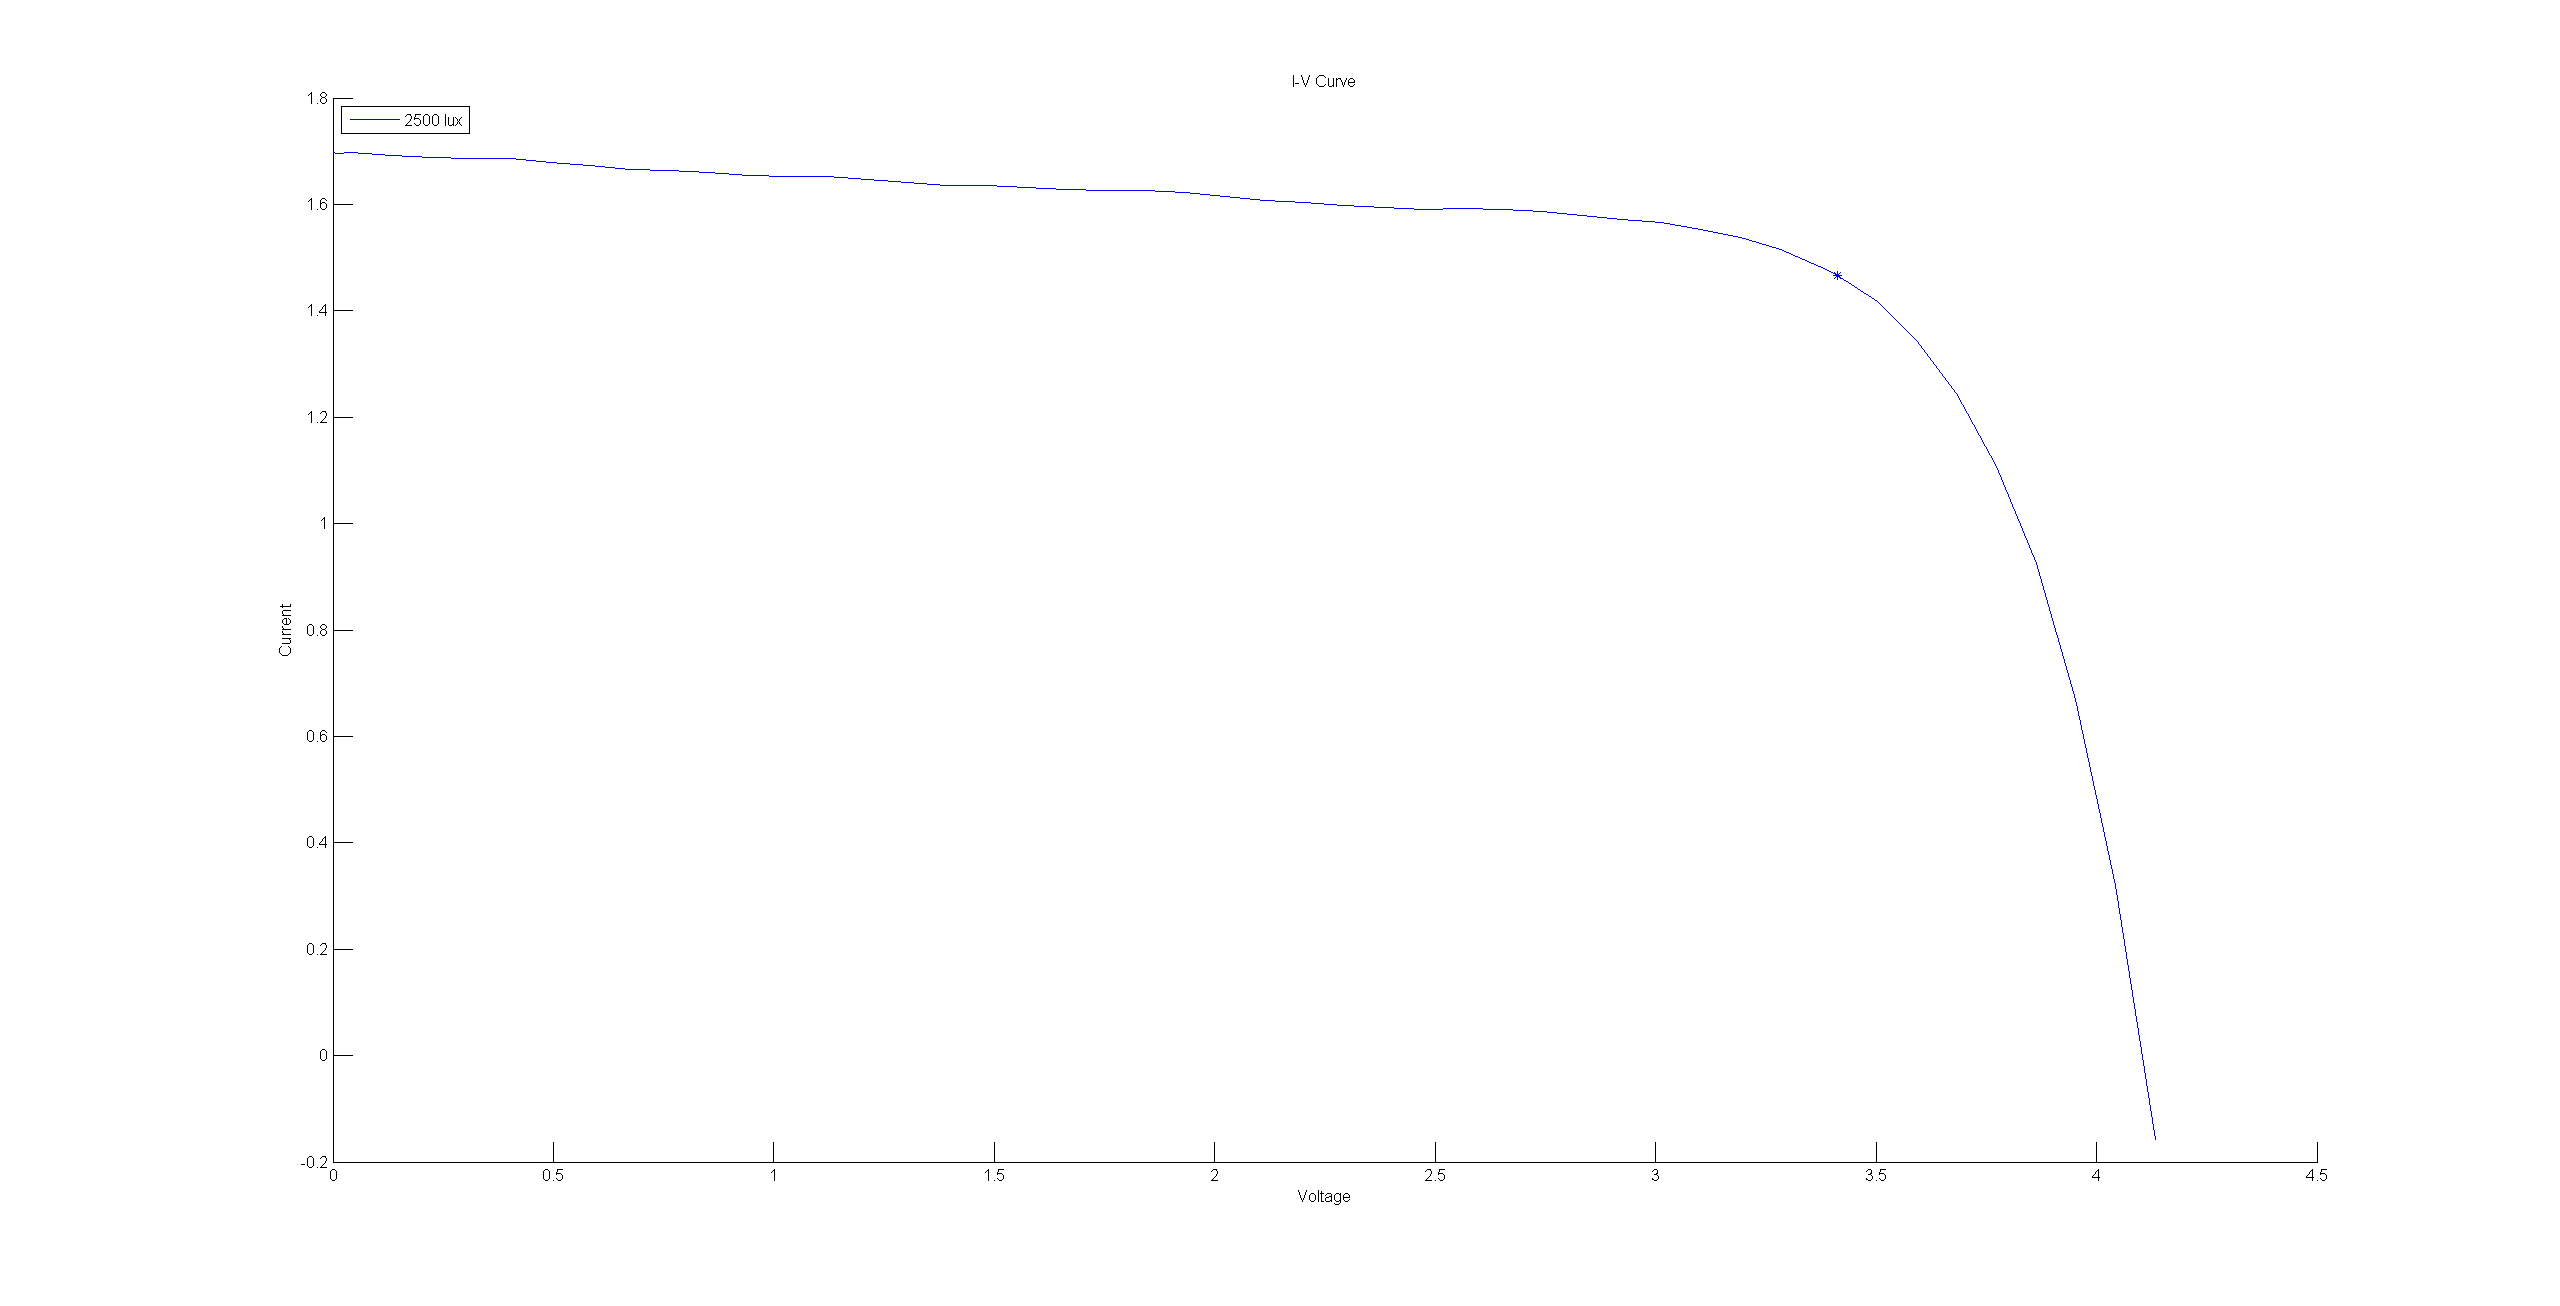
\includegraphics[width=\textwidth]{images/single2500_IV}
  \caption{I-V curve for the array at steady illumination}
  \label{fig:2500luxIV}
  \end{center}
  \end{figure}
  
\begin{figure}[H]
  \begin{center}
  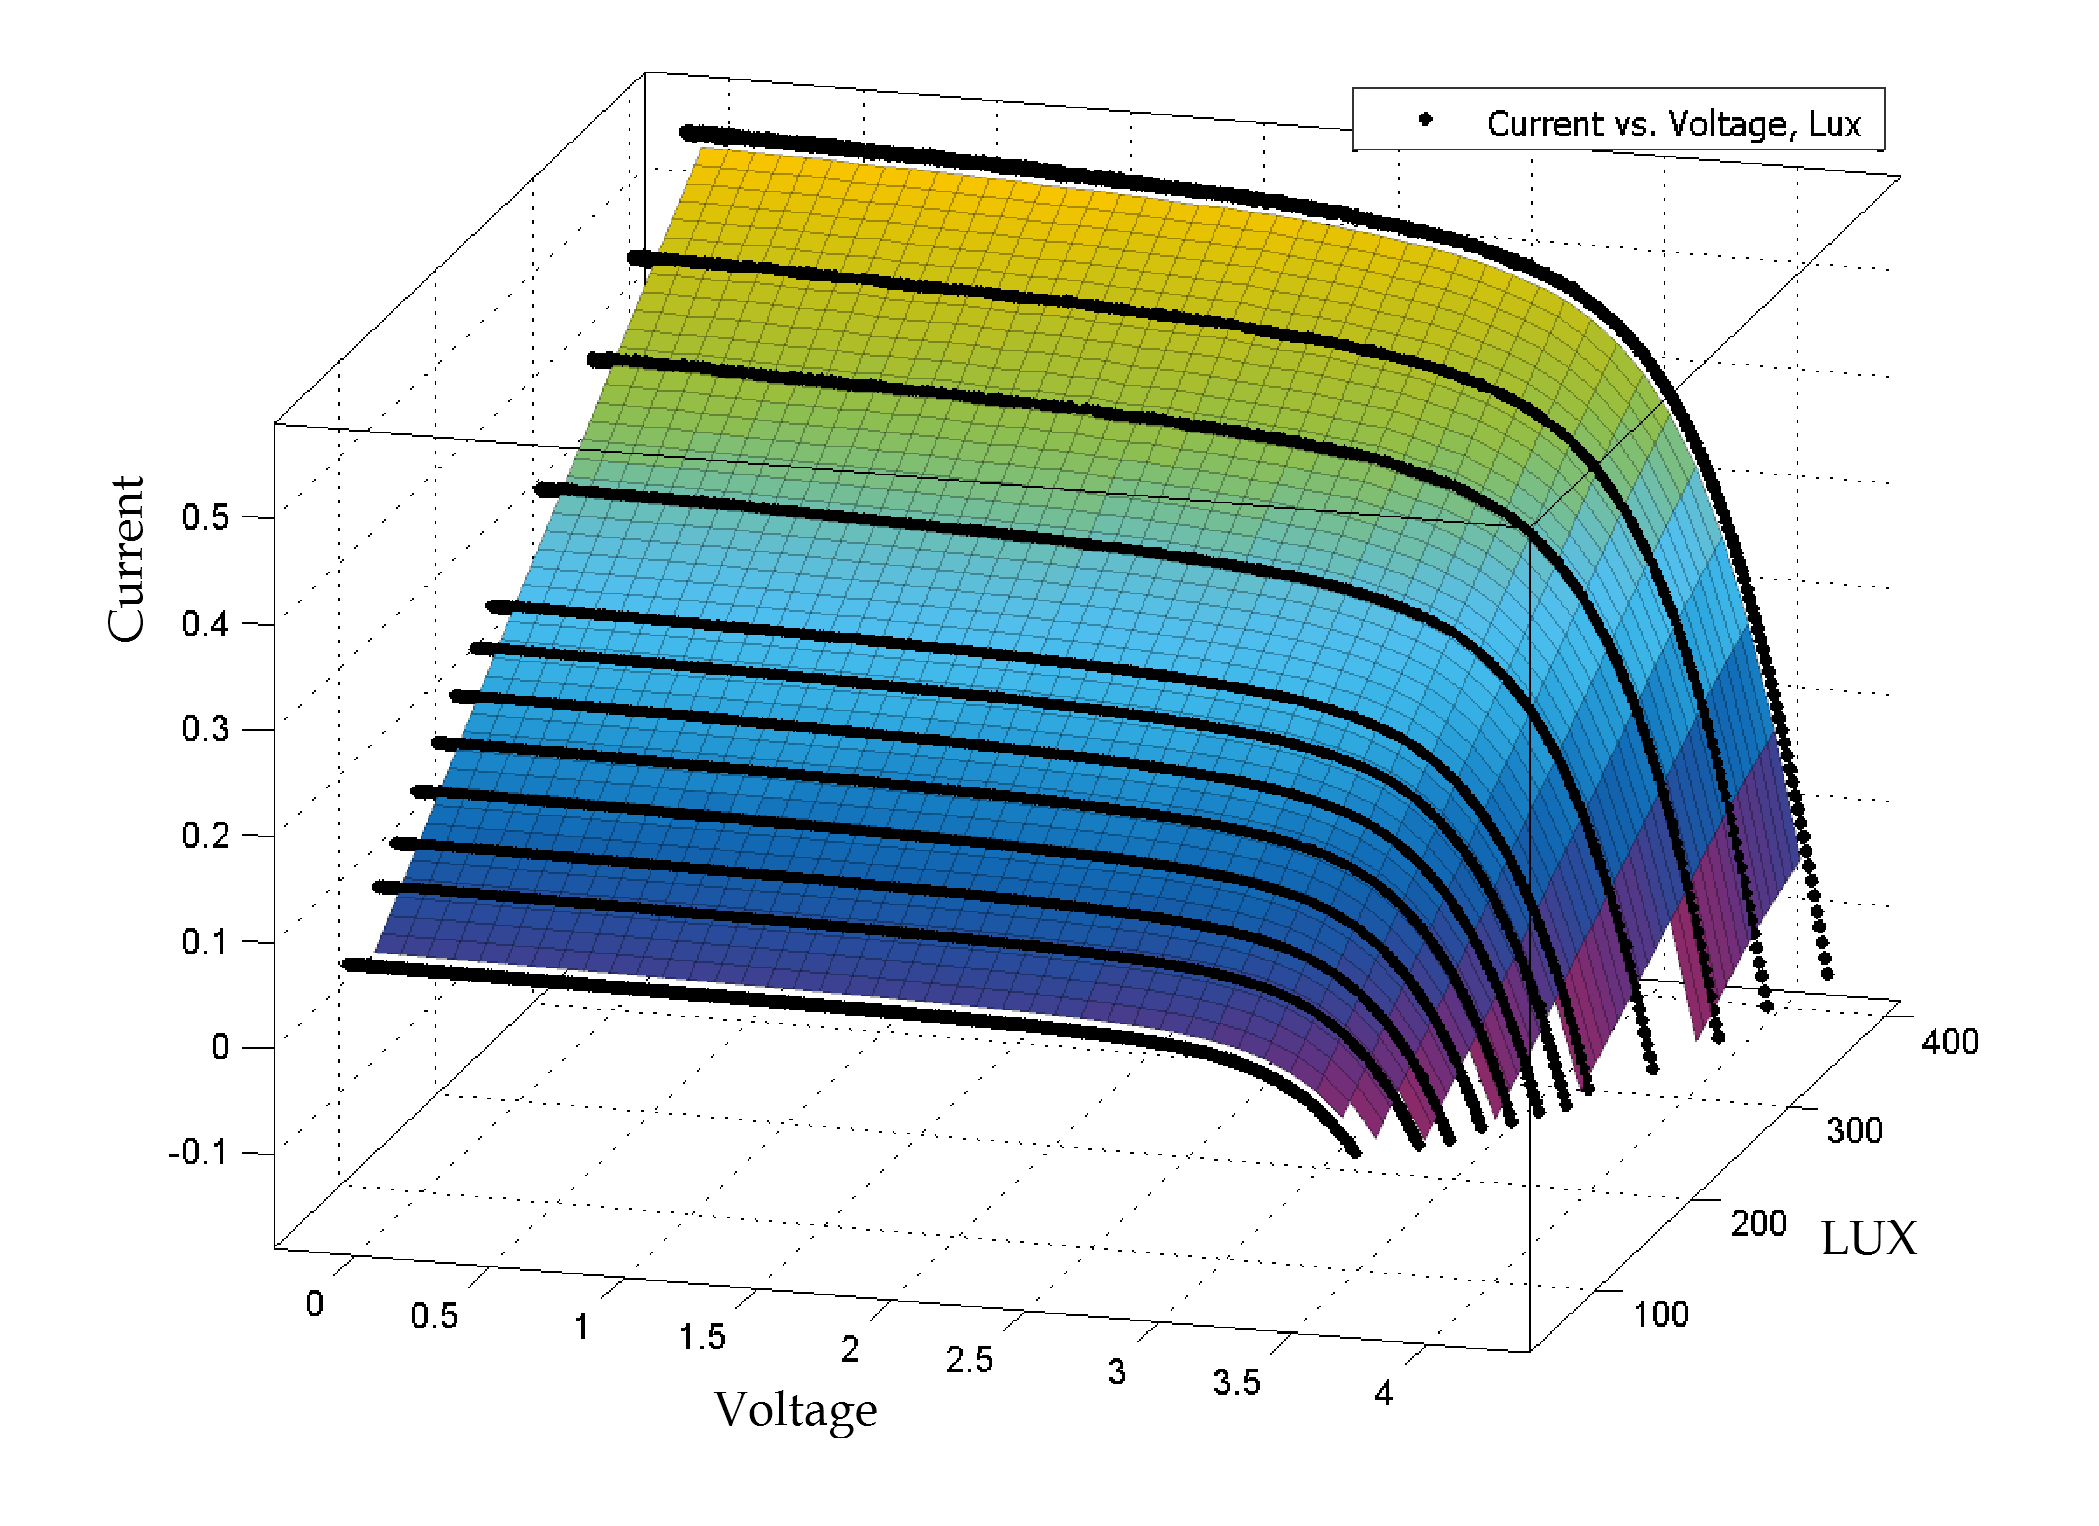
\includegraphics[width=\textwidth]{images/I-V-lux}
  \caption{I-V curve for the array at varying illumination}
  \label{fig:luxIV100_2500}
  \end{center}
  \end{figure}

\section{Modelling and Simulations} 

\begin{figure}[H]
  \begin{center}
  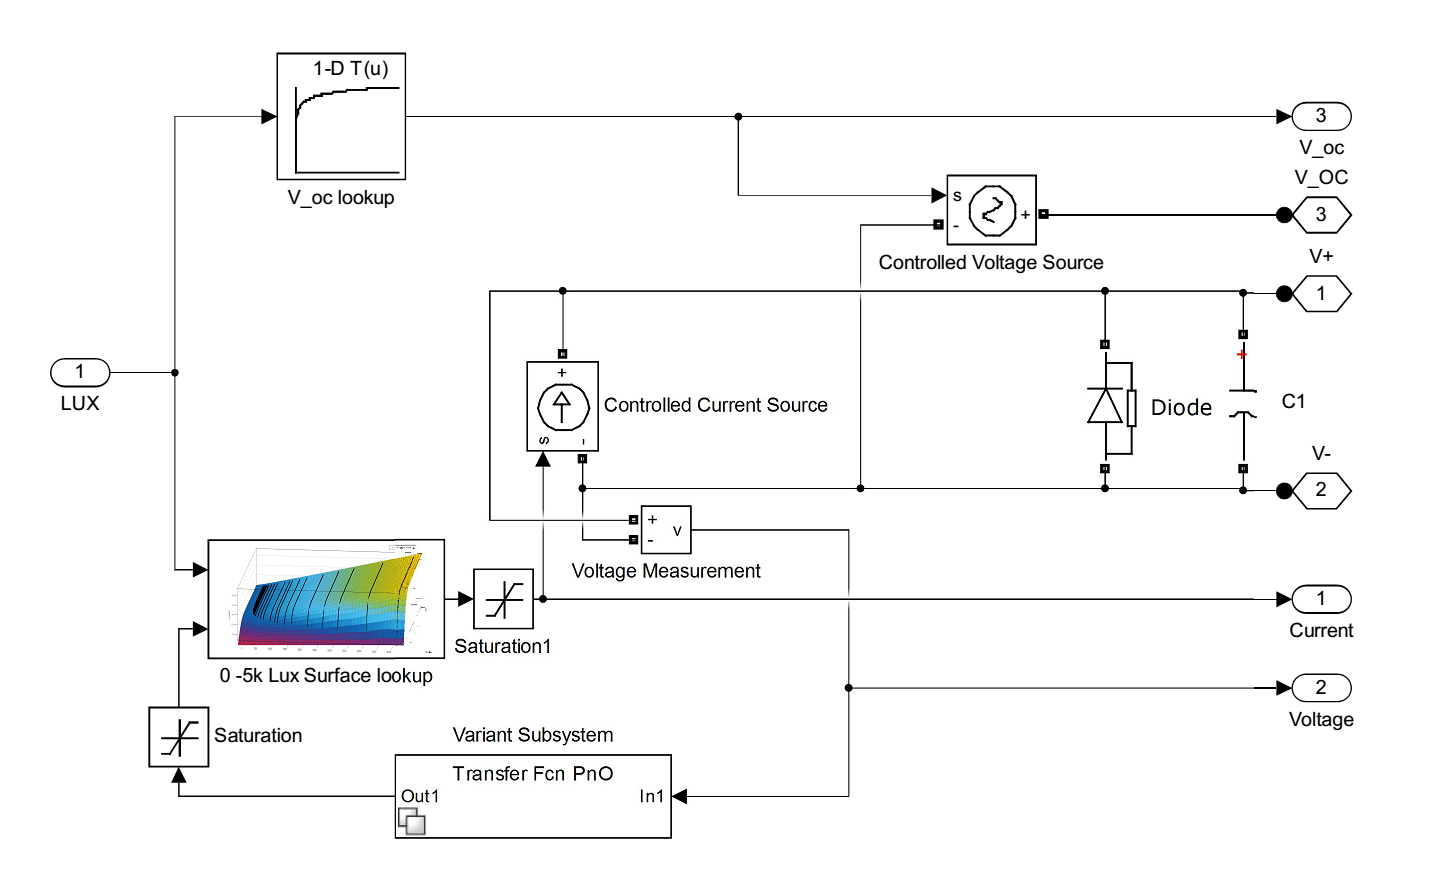
\includegraphics[width=\textwidth]{images/PV_block_Model}
  \caption{Modelling of the DSC Subsystem }
  \label{fig:PV_block_Model}
  \end{center}
  \end{figure}

\begin{figure}[H]
  \begin{center}
 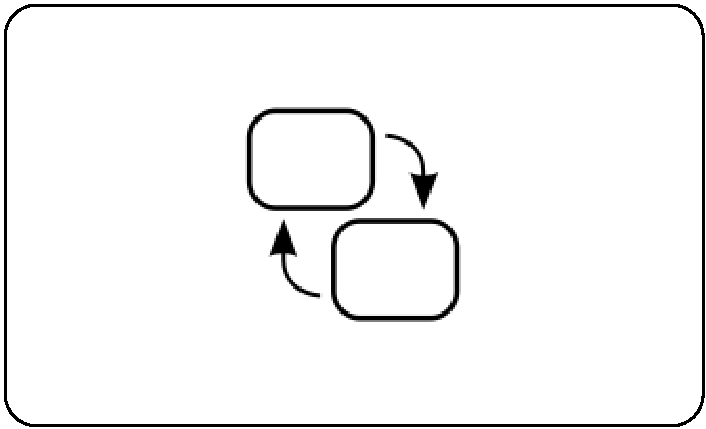
\includegraphics[width=\textwidth]{images/IC_stateflow}
  \caption{Top Model }
  \label{fig:Model_top}
  \end{center}
  \end{figure}

 \begin{figure}[H]
  \begin{center}
	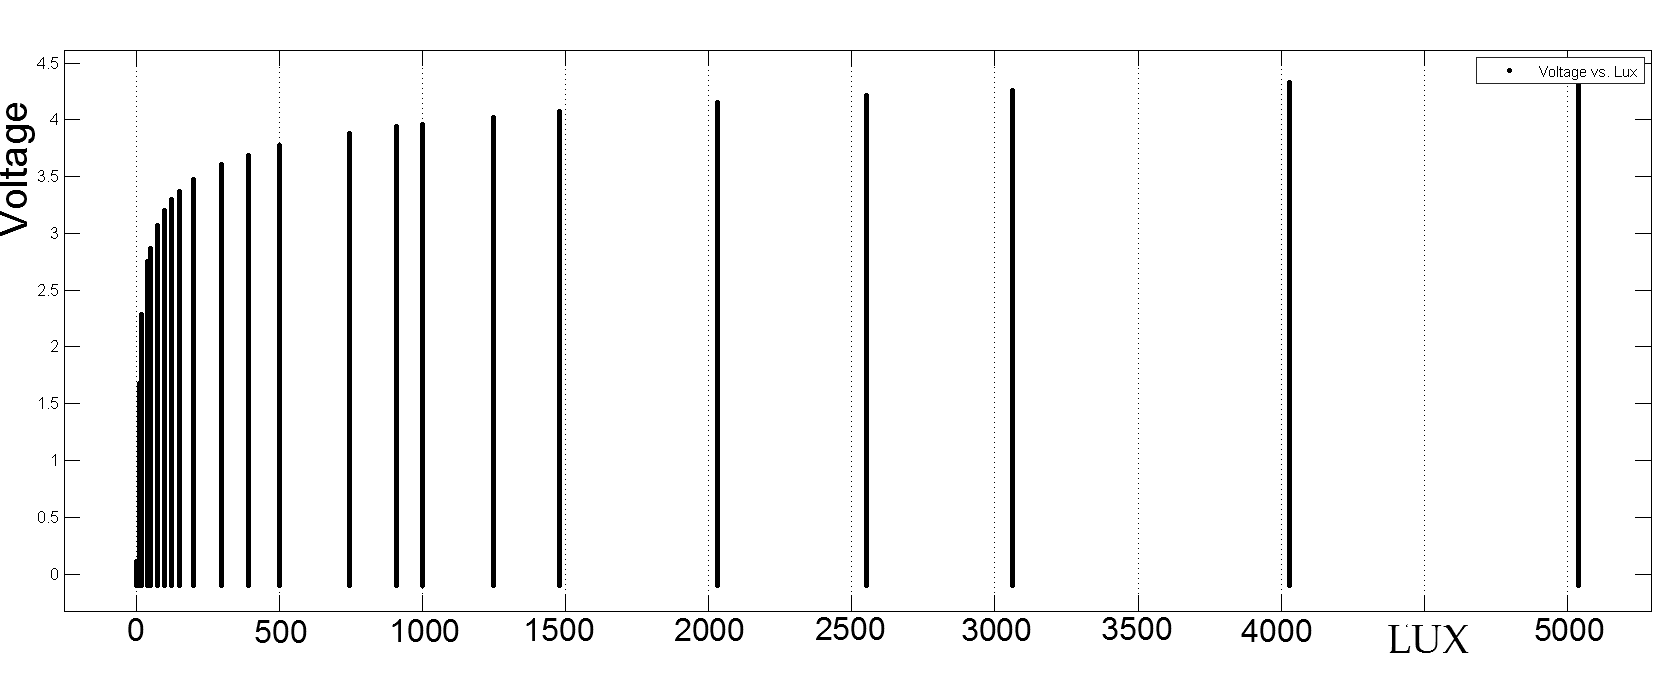
\includegraphics[width=\linewidth]{images/Voltagevlux}
	\caption{spread of measured illumination vs Voltage  }
	\label{fig:Voltagevlux}
  \end{center}
 \end{figure}
 
However due to the near impossibility of accurately measuring all the variables of a unknown cell for this research work,a model was constructed by placing a the test cell under a battery of varied illuminations (0 Lux - 5050 Lux) shown in figure ~\ref{fig:Voltagevlux} . Which resulted in a surface that closely resembles the cell's operation in real world conditions. particular attention was paid to low light conditions which is to be expected for indoor illuminations ( < 2000 Lux).As \ac{DSCs} display are very stable output across a large temperature range, the above model was made independent of temperature variations. 


\section {Validation in Matlab{\textregistered}}

text text text text text text text text text text text text text text text text text text text text text text text text text text text text text text text text text text text text text text text text text text text text text text text text text text text text text text text text text text text text text text text text text text text text text text  \\



insert text here insert text here insert text here insert text here insert text here
insert text here insert text here insert text here insert text here insert text here insert text here insert text here insert text here insert text here insert text here insert text here insert text here insert text here insert text here insert text here insert text here insert text here insert text here insert text here insert text here insert text here insert text here insert text here insert text here   \\

insert text here insert text here insert text here insert text here insert text here
insert text here insert text here insert text here insert text here insert text here insert text here insert text here insert text here insert text here insert text here insert text here insert text here insert text here insert text here insert text here insert text here insert text here insert text here insert text here insert text here insert text here insert text here insert text here insert text here   \\




\begin{figure}[H]
  \begin{center}
  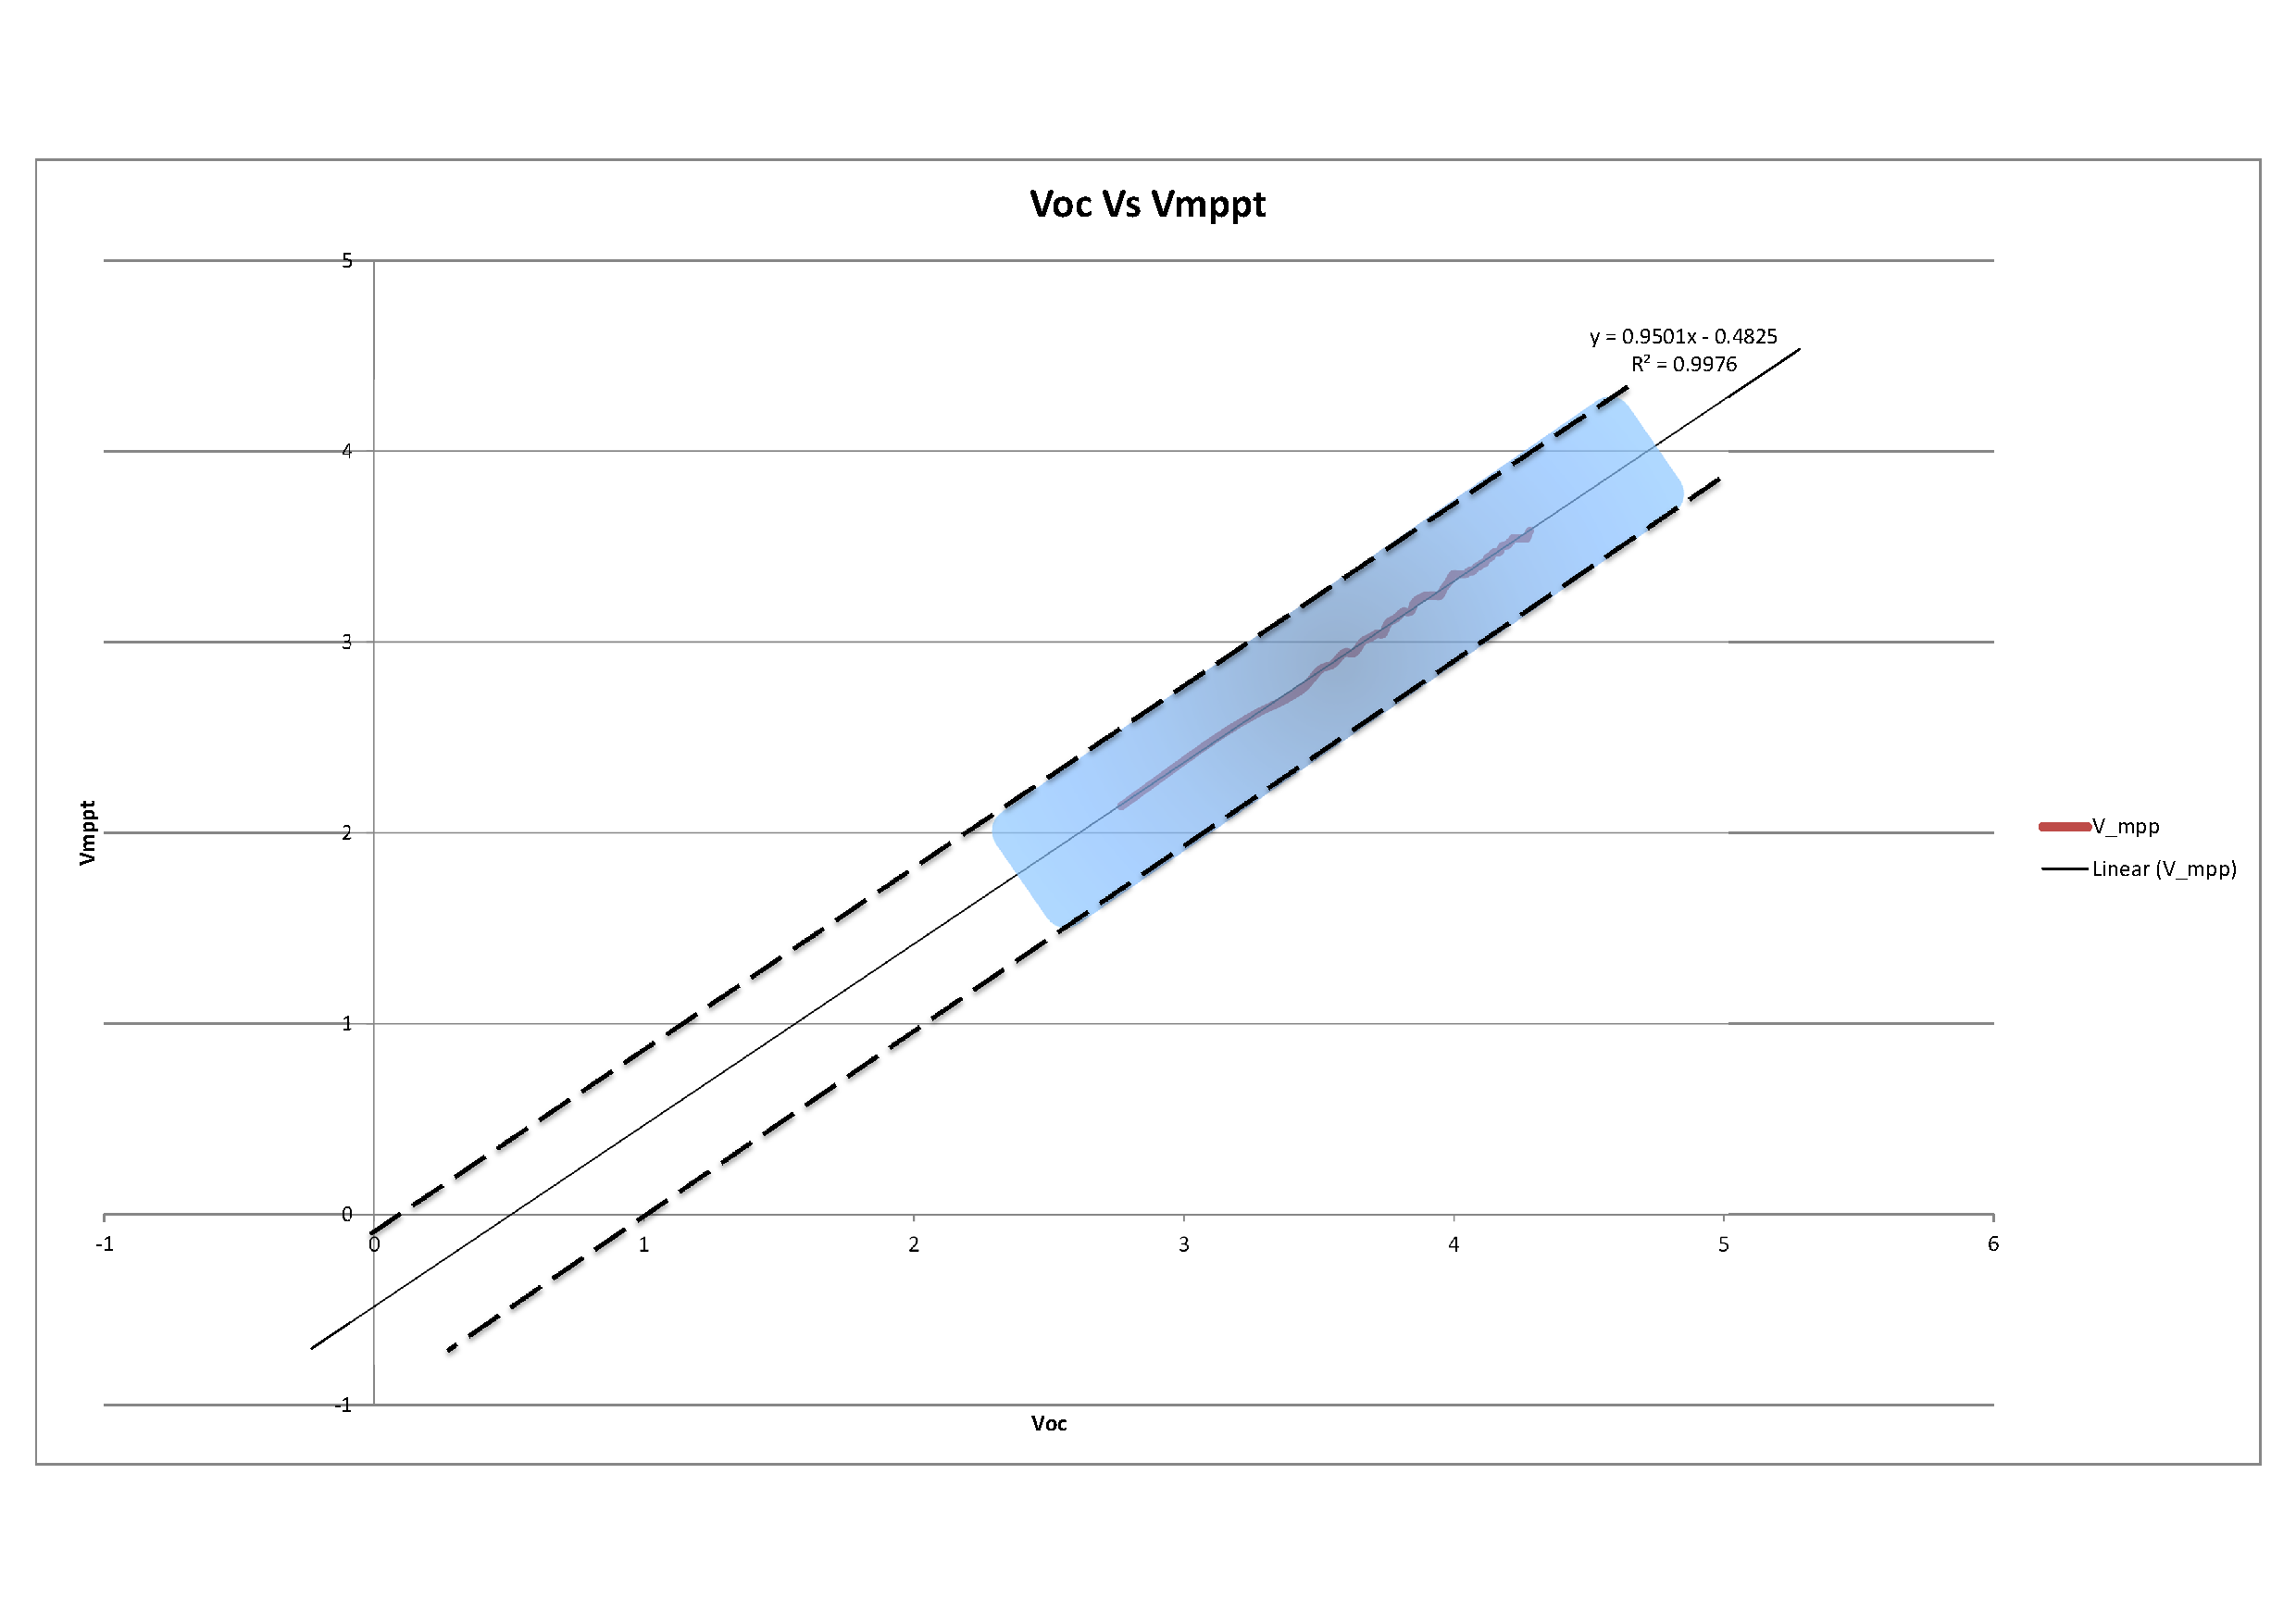
\includegraphics[width=1.1\textwidth]{images/Probability_field}
  \caption{Probability field }
  \label{fig:Probability_field}
  \end{center}
\end{figure}

  \begin{figure}[H]
   \begin{center}
   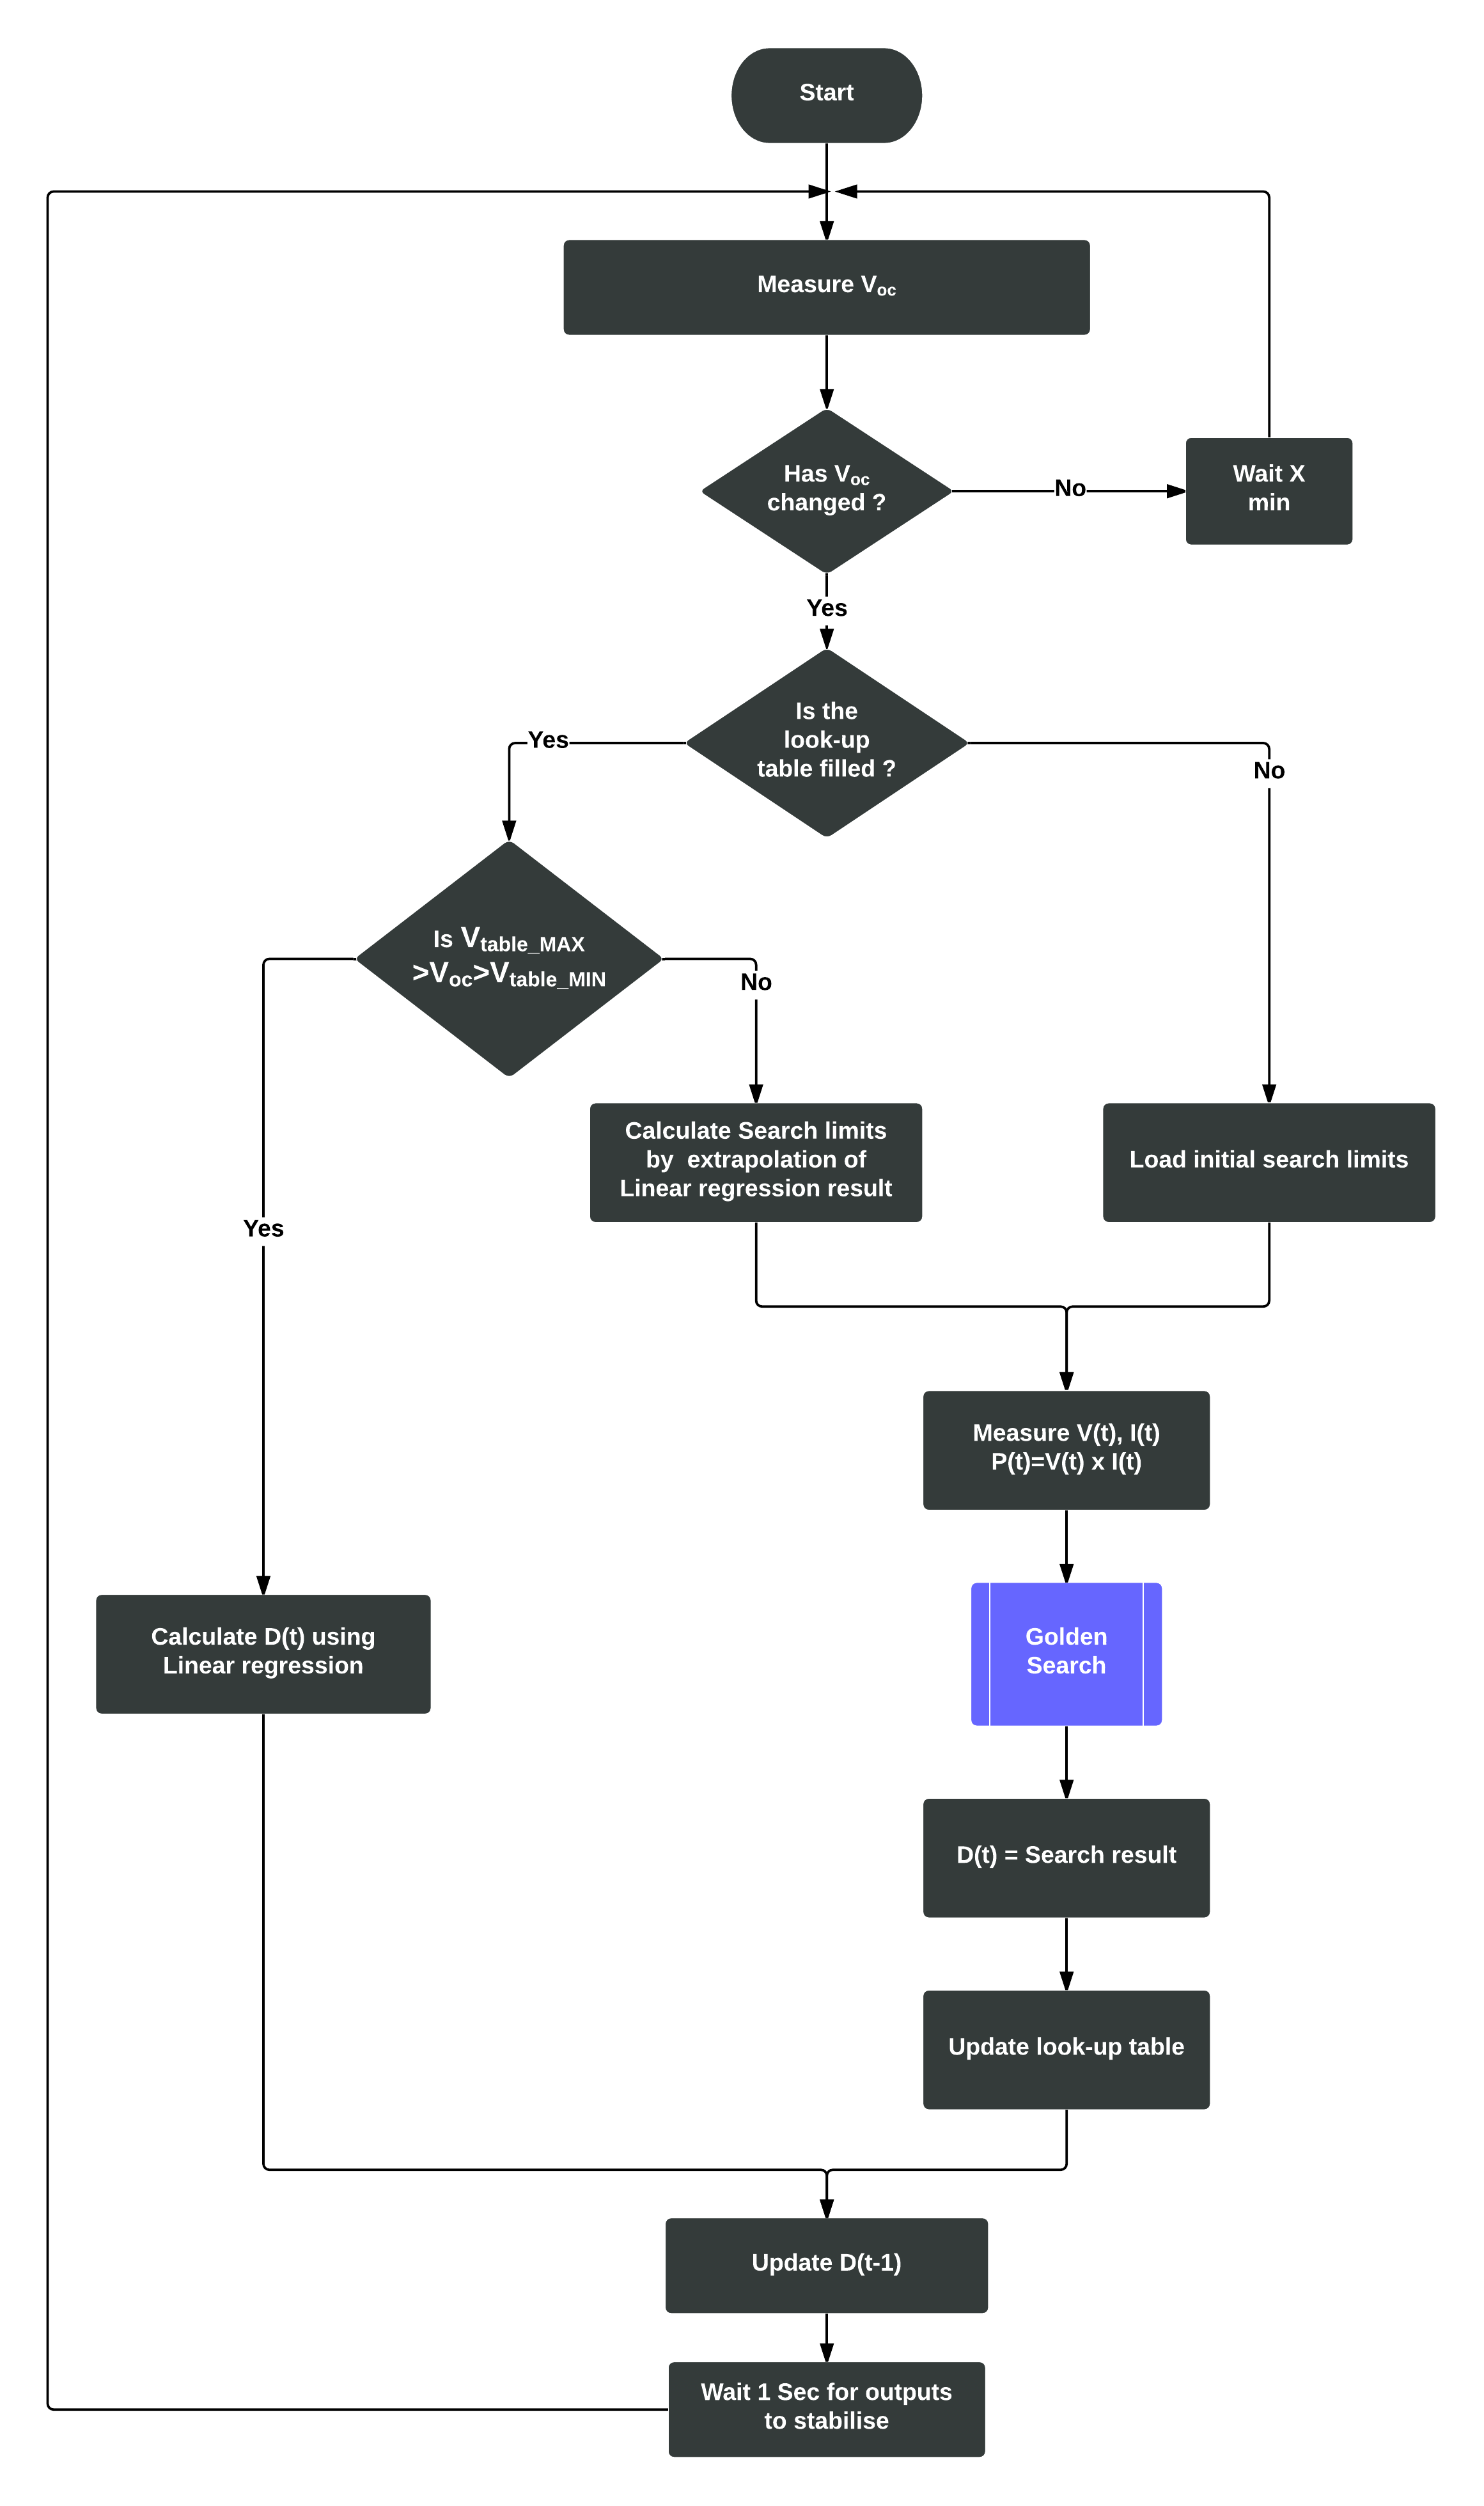
\includegraphics[width=0.9\textwidth]{images/Proposed_Flow}
   \caption{ Flow chart for Proposed MPPT Algorithm }
   \label{fig:cyflow}
   \end{center}
  \end{figure}





